\documentclass[11pt]{article}

% Make margins smaller
\usepackage[top=1.1in, bottom=1.1in, left=1.1in, right=1.1in]{geometry}
% more advanced mathematical symbols
\usepackage{amsfonts}
\usepackage{amssymb}
\usepackage{amsmath}
\usepackage{bm}
\usepackage{bold-extra} % bold texttt
\usepackage{graphicx}
\usepackage{enumerate}
\usepackage[font=small,labelfont=bf]{caption} % Required for specifying captions to tables and figures
\usepackage{pgfgantt} % gantt chart!

\graphicspath{ {./images/} }

\begin{document}

\title{\textbf{Machine Learning Summative}}
\date{for 22nd March 2019}
\author{wbbz74}
\maketitle 

\section{Image Classifier}

% MAYBE DON'T TREAT IT SO MUCH AS A NARATIVE AND DON'T SHOW SO MANY GRAPHS OF THE PERFORMANCE? JUST TALK ABOUT SPECIFIC THINGS THAT DID/DIDN'T WORK

The base network consists of a simple, 3 layer fully connected network containing only 1 hidden layer. This performs poorly as there is little opportunity for the network to learn deep and abstract representations by using a single hidden layer. Additionally, spatially related information is not considered together---a vital aspect of an image classification task, where neighbouring pixels need to be considered as a unit in order to identify items in given images. After around 50 epochs, this network only shows accuracy of around 15\%, also showing signs of overfitting as the training becomes better classified than the test set.

    \begin{center}
        \begin{minipage}{0.75\linewidth}
            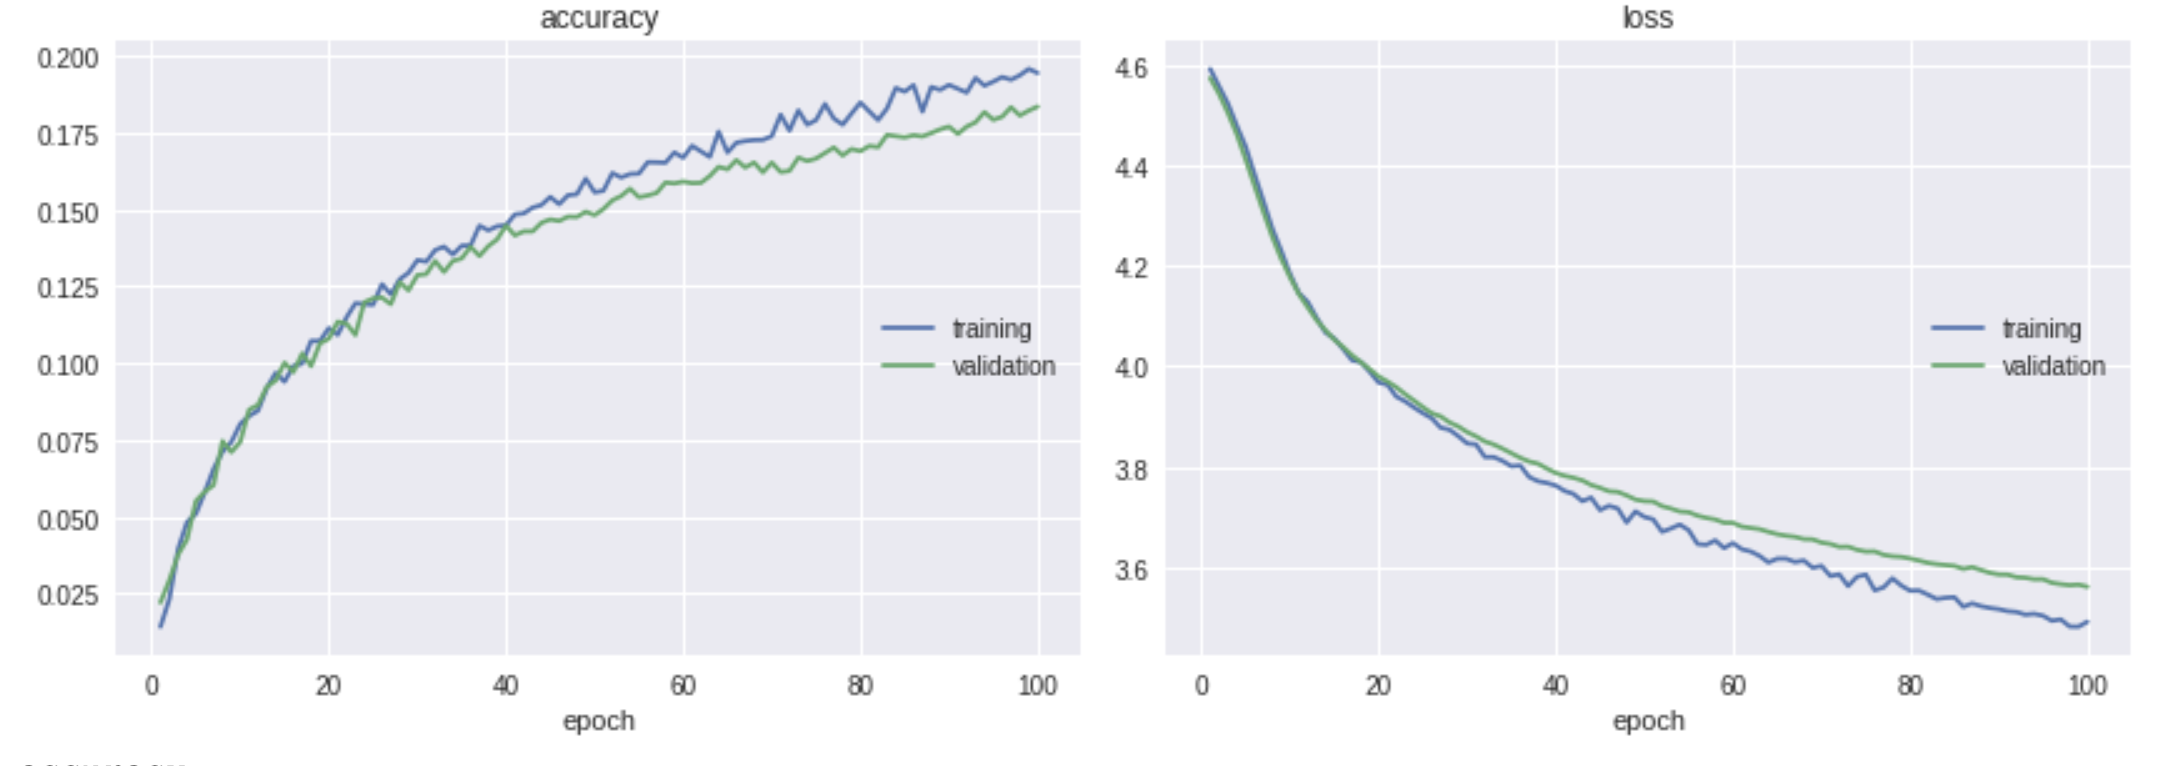
\includegraphics[width=\linewidth]{accuracy0}
            \captionof{figure}{Initial accuracy, 3 fully connected layers (1 hidden) with ReLU normalisation.}
        \end{minipage}%
    \end{center}


To remedy this, we replace the pure linear structure of the network with a convolution based network. Convolutional Neural Networks (CNNs) are able to better learn representations based on a number of spatially related inputs, allowing for better generalisation of image data. This is achieved by learning convolution masks and which reduce the dimensionality of the image. 

My first modified network consisted of 2 convolutional layers, each followed by a max pooling layer (2x2). Then, flattening this output, it is passed to two hidden fully-connected layers before the final classification layer. As shown in Figure \ref{fig:first-conv}, after 100 epochs the network shows far fewer signs of overfitting as the accuracy climbs past 20\%.

\begin{small}
\begin{verbatim}
class BetterNetwork(nn.Module):

    def __init__(self):
        super(BetterNetwork, self).__init__()
        self.conv1 = nn.Conv2d(3,6,5)
        self.pool1 = nn.MaxPool2d(2,2)
        self.conv2 = nn.Conv2d(6,12,3)
        self.pool2 = nn.MaxPool2d(2,2)
        self.fc1 = nn.Linear(in_features=432, out_features=512)
        self.fc2 = nn.Linear(in_features=512, out_features=100)

    def forward(self, x):
        x = self.pool1(F.relu(self.conv1(x)))
        x = self.pool2(F.relu(self.conv2(x)))
        x = x.view(x.size(0), -1) # flatten
        x = self.fc1(x)
        x = self.fc2(x)
        return x
\end{verbatim}
\end{small}


    \begin{center}
        \begin{minipage}{0.75\linewidth}
            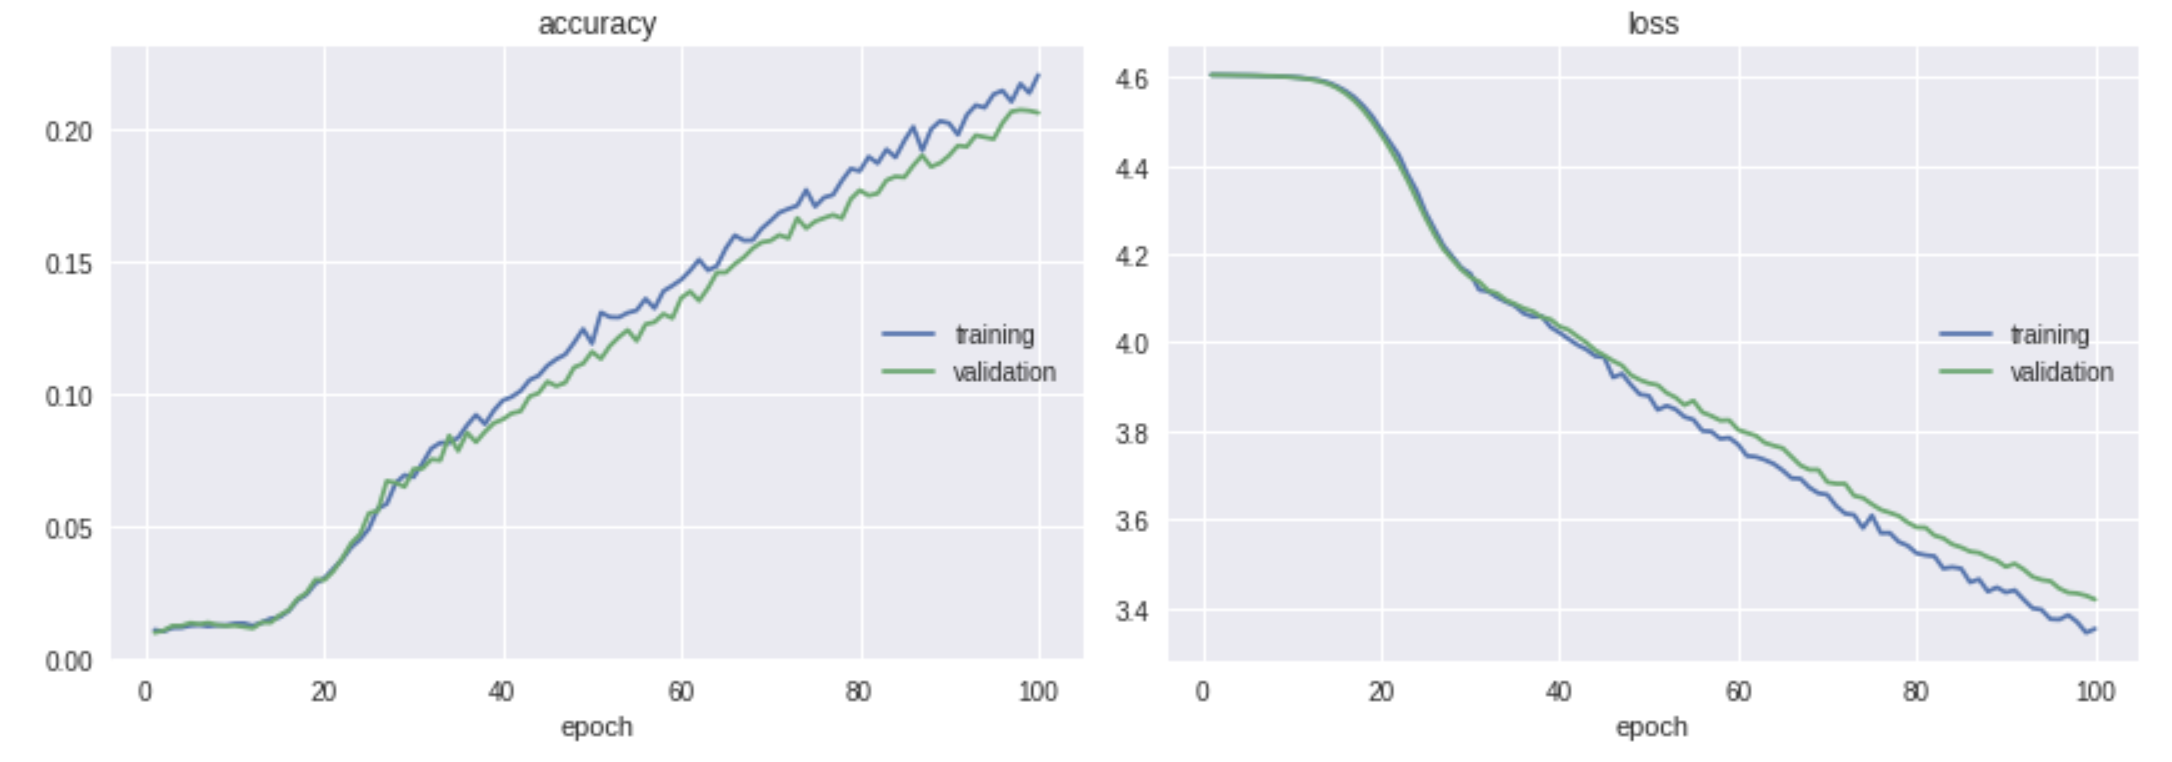
\includegraphics[width=\linewidth]{accuracy1}
            \captionof{figure}{Initial convolution based network (2 conv2d layers, 2 maxpooling, 2 fully-connected layers.}
            \label{fig:first-conv}
        \end{minipage}%
    \end{center}


In order to try and obtain better results from the existing network, I increased the batch size from 16 to 32. This should allow for better generalisations to be learned at once, as more training examples will now be considered before weights and biases are updated at each step. Additionally, I added an additional convolutional layer, as well as using a max pooling layer on each of these. Thus our current network architecture is:

\begin{center}
\begin{small}
\begin{verbatim}
class MyNetwork(nn.Module):

    def __init__(self):
        super(MyNetwork, self).__init__()
        self.conv1 = nn.Conv2d(3,6,3)
        self.pool1 = nn.MaxPool2d(2, 2)
        self.conv2 = nn.Conv2d(6,16,3)
        self.pool2 = nn.MaxPool2d(2, 2)
        self.fc1 = nn.Linear(in_features=576, out_features=512)
        self.fc2 = nn.Linear(in_features=512, out_features=100)

    def forward(self, x):
        x = self.pool1(F.relu(self.conv1(x)))
        x = self.pool2(F.relu(self.conv2(x)))
        x = x.view(x.size(0), -1) # flatten
        x = self.fc1(x)
        x = self.fc2(x)
        return x
\end{verbatim}
\end{small}
\end{center}

Surprisingly, this gave much worse results than anything before, accuracy not even climbing past 2\%. However, as the accuracy had not seemed to level off as much as prior examples, I increased the number of epochs from 10 to 25, giving the network more opportunities to pick up features from the training data. This revealed something very remarkable---the best improvements to the network only started to be experienced after 10 epochs. Not seeing any signs of overfitting, I further increased the number of epochs to 50, and was able to see further improvements still.

  \begin{center}
        \begin{minipage}{0.48\linewidth}
            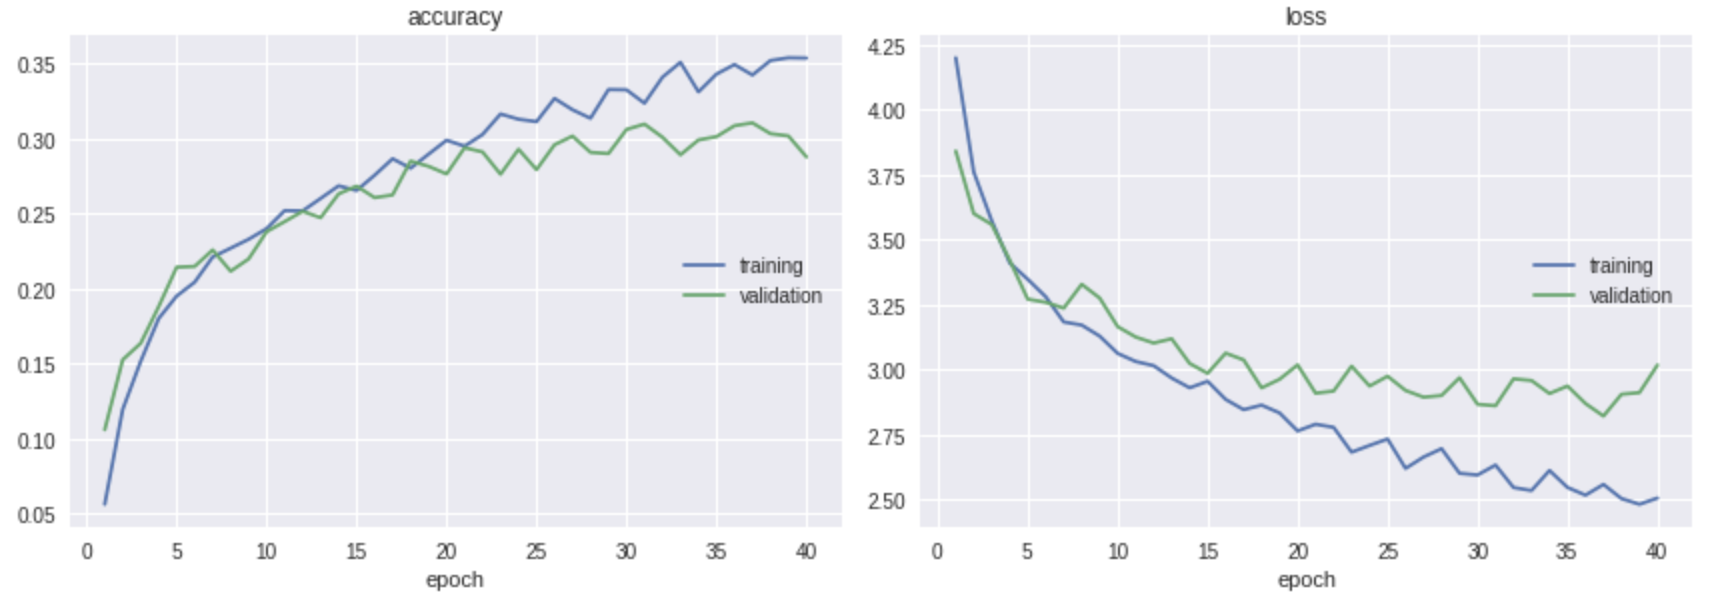
\includegraphics[width=\linewidth]{accuracy4}
            \captionof{figure}{25 epochs, accuracy still rapidly climbing---notice no improvements until after 10 epochs}
            \end{minipage}%
            \hfill
            \begin{minipage}{0.49\linewidth}
            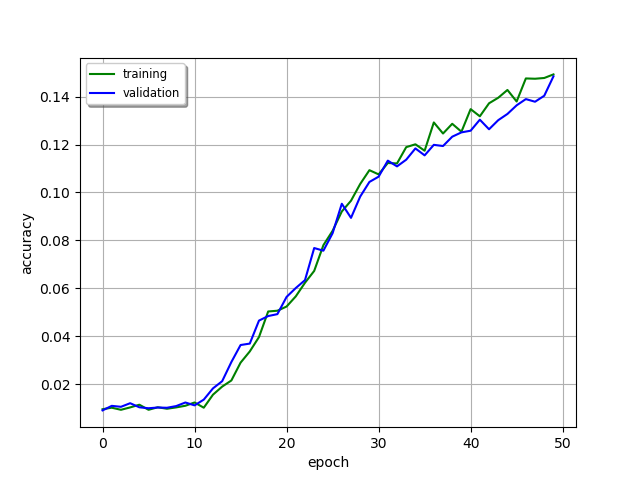
\includegraphics[width=\linewidth]{accuracy5}
            \captionof{figure}{50 epochs, still no signs of overfitting}
        \end{minipage}
    \end{center}


\section{Generating a Pegasus}


\end{document}